A rather rare $\mathbf{k} \cdot \mathbf{p}$ question!
Still pretty doable if you stick to the basic principles of perturbation theory.

\begin{parts}
	\part From Bloch's theorem,
	\begin{align*}
		\psi_{n\mathbf{k}} (\mathbf{r} + \mathbf{R}) &= \psi_{n\mathbf{k}} (\mathbf{r}) \\
		\Rightarrow \underbracket{\bcancel{u_{n\mathbf{k}} (\mathbf{r} + \mathbf{R})}}_{u_{n\mathbf{k}} (\mathbf{r})\textnormal{ by definition}} \cancel{\mathrm{e}^{i\mathbf{k} \cdot \mathbf{r}}} \mathrm{e}^{i\mathbf{k} \cdot \mathbf{R}} &= \bcancel{u_{n\mathbf{k}} (\mathbf{r})} \cancel{\mathrm{e}^{i\mathbf{k} \cdot \mathbf{r}}} \\
		\Rightarrow \mathrm{e}^{i\mathbf{k} \cdot \mathbf{R}} &= 1
	\end{align*}
	Hence $\mathbf{k}$ must be a reciprocal lattice vector.
	
	\part From the Hamiltonian $\mathcal{H} = p^2 / 2m + V(\mathbf{r})$, we have by TISE:
	\begin{align*}
		\frac{1}{2m} \left(-i\hbar\nabla\right) \left[\left(-i\hbar\nabla\right) \left(u_{n\mathbf{k}} \mathrm{e}^{i\mathbf{k} \cdot \mathbf{r}}\right)\right] + V(\mathbf{r}) u_{n\mathbf{k}} \mathrm{e}^{i\mathbf{k} \cdot \mathbf{r}} &= E_{n\mathbf{k}} u_{n\mathbf{k}} \mathrm{e}^{i\mathbf{k} \cdot \mathbf{r}} \\
		\frac{-i\hbar\nabla}{2m} \left[-i\hbar\nabla u_{n\mathbf{k}} \mathrm{e}^{i\mathbf{k} \cdot \mathbf{r}} + \hbar u_{n\mathbf{k}} \mathbf{k} \mathrm{e}^{i\mathbf{k} \cdot \mathbf{r}}\right] + \ldots &= \ldots \\
		\frac{1}{2m} \left[\left(-i\hbar\nabla\right)^2 u_{n\mathbf{k}} \cancel{\mathrm{e}^{i\mathbf{k} \cdot \mathbf{r}}} + 2\hbar u_{n\mathbf{k}} \mathbf{k} \cancel{\mathrm{e}^{i\mathbf{k} \cdot \mathbf{r}}} + \hbar u_{n\mathbf{k}} k^2 \cancel{\mathrm{e}^{i\mathbf{k} \cdot \mathbf{r}}}\right] + \ldots &= \ldots \\
		\Rightarrow \left[\frac{\left(\mathbf{p} + \hbar \mathbf{k}\right)^2}{2m} + V(\mathbf{r})\right] u_{n\mathbf{k}} &= E_{n\mathbf{k}} u_{n\mathbf{k}}
	\end{align*}
	
	\part We want perturbation so we recast the Hamiltonian in the following form:
	\begin{align*}
		\mathcal{H} &= \mathcal{H}_0 + \lambda \Delta \mathcal{H} \\
		&= \left[\frac{p^2}{2m} + V(\mathbf{r})\right] + \frac{\lambda}{2m} \left[2\hbar \mathbf{k} \cdot \mathbf{p} + \hbar^2 k^2\right]
	\end{align*}
	
	\part From perturbation theory we have the 1st order energy shift as:
	\begin{align*}
		\Delta E^{(1)} &= \bra{u_{20}} \Delta \mathcal{H} \ket{u_{20}} \\
		&= \cancelto{0}{\bra{u_{20}} \frac{\hbar \mathbf{k}\cdot\mathbf{p}}{m} \ket{u_{20}}} \;\;+\; \bra{u_{20}} \frac{\hbar^2 k^2}{2m} \ket{u_{20}} \\
		&= \frac{\hbar^2 k^2}{2m}
	\end{align*}
	
	2nd order energy shift:
	\begin{align*}
		\Delta E^{(2)} &= \sum_{n \neq 2} \frac{\left|\bra{u_{n0}} \Delta \mathcal{H} \ket{u_{n0}}\right|^2}{E_{20} - E_{n0}} \\
		&= \frac{\left|\bra{u_{10}} \Delta \mathcal{H} \ket{u_{20}}\right|^2}{E_{20} - E_{10}} \textnormal{\hspace{1em}for a 2-band, isotropic semiconductor} \\
		&= \frac{\left|\bra{u_{10}} \dfrac{\hbar \mathbf{k} \cdot \mathbf{p}}{m} \ket{u_{20}}\right|^2}{E_g} \textnormal{\hspace{1em}where $E_g$ is the band gap} \\
		&= \frac{\hbar^2 k^2}{m^2} \cdot \frac{1}{E_g} \cdot P_{12}
	\end{align*}
	
	So to 2nd order,
	\begin{align*}
		E_{2\mathbf{k}} &= E_{20} + \frac{\hbar^2 k^2}{2m} + \frac{\hbar^2 k^2}{m^2} \cdot \frac{P_{12}}{E_g} \\
		&= E_{20} + \frac{\hbar^2 k^2}{2m} \left[1 + 2\frac{P_{12}}{m E_g}\right]
	\end{align*}
	
	\part From above,
	\begin{align*}
		\frac{\partial^2 E}{\partial k^2} &= \frac{\hbar^2}{m} \left[1 + 2\frac{P_{12}}{E_g}\right] = \frac{\hbar^2}{m^*} \\
		\Rightarrow \frac{1}{m^*}
		&\propto \frac{1}{E_g}
	\end{align*}
	
	For holes, we repeat the perturbation from $u_{10}$ instead so we have $\Delta E^{(2)} \rightarrow -\Delta E^{(2)}$.
	
	Hence:
	\begin{align*}
		\frac{1}{m_h^*} &= \frac{1}{m} \left[1 - 2\frac{P_{12}}{E_g}\right] \\
		&\propto -\frac{1}{E_g}
	\end{align*}
	
	We may illustrate the difference in sign by inspecting the structure of an isotropic quadratic band:
	\begin{figure}[H]
		\centering
		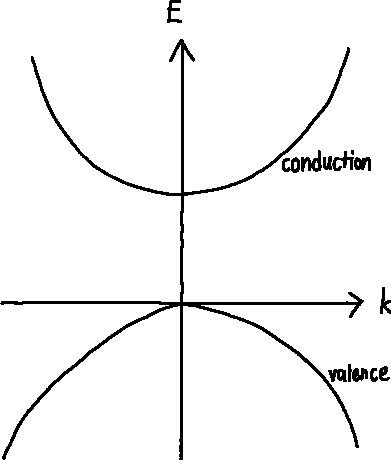
\includegraphics{q2-band-curvature}
	\end{figure}
	Since the effective mass is defined with respect to the 2nd derivative of a band, it is clear that the only difference between the conduction and valence band here is the sign of the slope, hence the sign difference in effective mass.
\end{parts}